%-----General Settings----%
\documentclass{other/docTemplate}
\svnid{$Id$}

\author{ML: Gonzalo Ducca \formatemail{gonzaloducca@gmail.com} \\ DA: Juan P. Bertone \formatemail{bertonejpb@gmail.com} \\ DE: Juan E. Flórez-Coronel \formatemail{juan.florez@upr.edu} \\ DA: Valentino Caputa \formatemail{caputavalentino@gmail.com} \\ ML: Carlos Madoery \formatemail{ccmadoery@gmail.com}}  
\po{Melina Griffo \formatemail{meligriffo@gmail.com}}
\title{Reporte del Proyecto Final: Expectativa de vida} 
\henrymentor{Pía Ruiz \formatemail{mpiaruiz@gmail.com}}

\loadglsentries{other/acronyms}
\makeglossaries

%-----Beginning of Document----%
\begin{document} 
\maketitle

%---Revision Tracker---%
\startTable
\AddRevision{0.0}{10-20-23}{Creación del documento}
\AddRevision{1.0}{11-01-23}{Documentación Sprint 1}
\AddRevision{2.0}{11-15-23}{Documentación Sprint 2}
\stopTable

%-----Table of Contents-----%
\tableofcontents
\newpage
\listoftables
\newpage
\listoffigures
\newpage
\printglossary[title=Lista de Acronimos ,type=\acronymtype]
\clearpage

%-----Acknowledgments-----%
%\section*{Acknowledgments}
%\addcontentsline{toc}{section}{Acknowledgments}%adds acknowledgements section to the table of contents

%Here is a sample for how to susse acronyms. "Defining a \gls{fr} and a \gls{ps} provides a language for system design. This language is an important aspect of \gls{csd}."
%\newpage

%-----Abstract-----%
%\section*{Abstract}
%\addcontentsline{toc}{section}{Abstract}%adds Abstract section to the table of contents
%\newpage

%-----Content-----%
%%%%%%   PLANTEAMIENTO DEL PROBLEMA  %%%%%%                                               
\section{Planteamiento del problema}
Consultamos bases de datos del Banco Mundial y decidimos utilizar como referencia temas clave que proporcionan indicadores que influyen en la esperanza de vida de los habitantes de un país. Estos temas seleccionados son la educación, la salud, la economía, el desarrollo de la ciencia y la tecnología y el ámbito social.
Planeamos recopilar indicadores de cada tema, crear las bases de datos con las que queremos trabajar y luego vincular estas variables para establecer relaciones. Visualizamos este proyecto como un producto que se puede ofrecer a una empresa que busque invertir en ciencia y desarrollo.
Una vez completado todo el trabajo de análisis de datos, crearemos modelos de aprendizaje automático especificando ciertos parámetros, como el porcentaje del PIB invertido en educación o ciencia. Estos modelos luego nos proporcionarán una esperanza de vida estimada para un país en particular.

%%%%%%  PLANTEAMIAENTO DEL PROBLEMA - Objetivos  %%%%%% 
\subsection{Objetivos}
Analizar la expectativa de vida en 30 paises en base a 5 factores:
\begin{itemize}
  \item Educación
  \item Salud
  \item Economía
  \item Ciencia y Tecnología
  \item Social
\end{itemize}

%%%%%%  PLANTEAMIENTO DEL PROBLEMA - Público objetivo  %%%%%% 
\subsection{Público objetivo}
El público obejtivo de este proyecto incluye entidades públicas y privadas con intereses creados en el tema y usuarios cotidianos que quieran conocer la esperanza de vida esperada en un país determinado. 
 Las instituciones públicas, como las agencias gubernamentales, pueden utilizar los conocimientos y modelos generados para informar decisiones políticas y asignar recursos de manera efectiva en áreas relacionadas con la educación, la atención médica y la investigación científica. Por otro lado, las empresas privadas, especialmente aquellas involucradas en industrias relacionadas con la ciencia y la tecnología, pueden beneficiarse de los hallazgos del proyecto al tomar decisiones de inversión e iniciativas de responsabilidad social corporativa. Este proyecto está dirigido a una amplia gama de organizaciones que buscan tomar decisiones informadas que impacten el bienestar y el desarrollo de los países.

%%%%%%   PLANTEAMIENTO DEL PROBLEMA - Alcance del proyecto %%%%%%  
\subsection{Alcance del proyecto}
El alcance del proyecto implica un análisis exhaustivo de la esperanza de vida en 30 países de todo el mundo durante los últimos 35 años. Este análisis abarcará cinco temas clave dentro de cada uno de los cinco factores influyentes, a saber, educación, salud, economía, ciencia y tecnología y ámbito social. El objetivo es proporcionar una visión detallada y basada en datos de los factores que afectan la esperanza de vida en estos países durante el período de tiempo especificado.
 El producto final incluirá un servicio web donde se pueda acceder a la información brindada por el análisis y un dashboard interactivo con insights claves para la interpretación de los datos. 


%%%%%%  Obtención de los datos %%%%%%  
\clearpage
\section{Obtención de los datos}
La información fue obtenida utilizando la siguiente API \href{https://datahelpdesk.worldbank.org/knowledgebase/topics/125589}{World Bank API}.

%%%%%%   API %%%%%%  

\subsection{World Bank API}

La información de la API de World Bank tiene los siguientes tópicos:

\begin{figure}[htbp!]
  \centering
  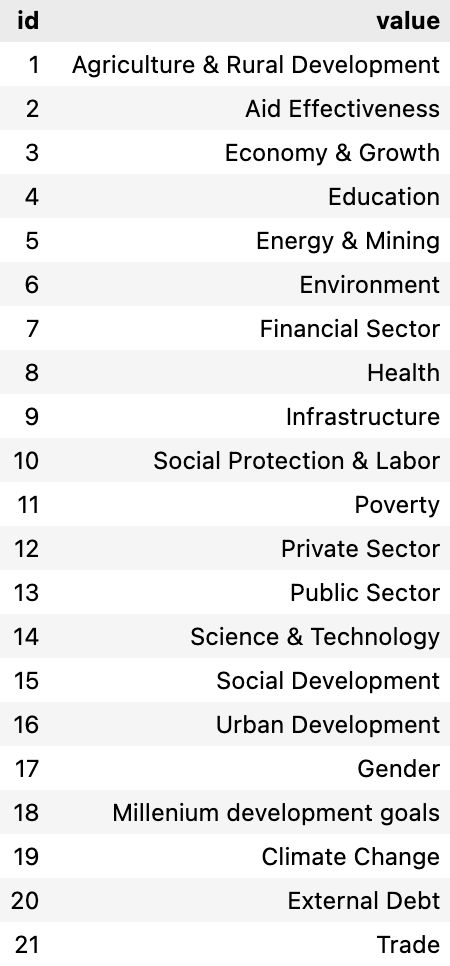
\includegraphics[width=0.4\textwidth]{topics.png}
  \caption{Tópicos World Bank}
  \label{fig:topics}
\end{figure}

\newpage

Y las siguientes economías:

\begin{figure}[htbp!]
  \centering
  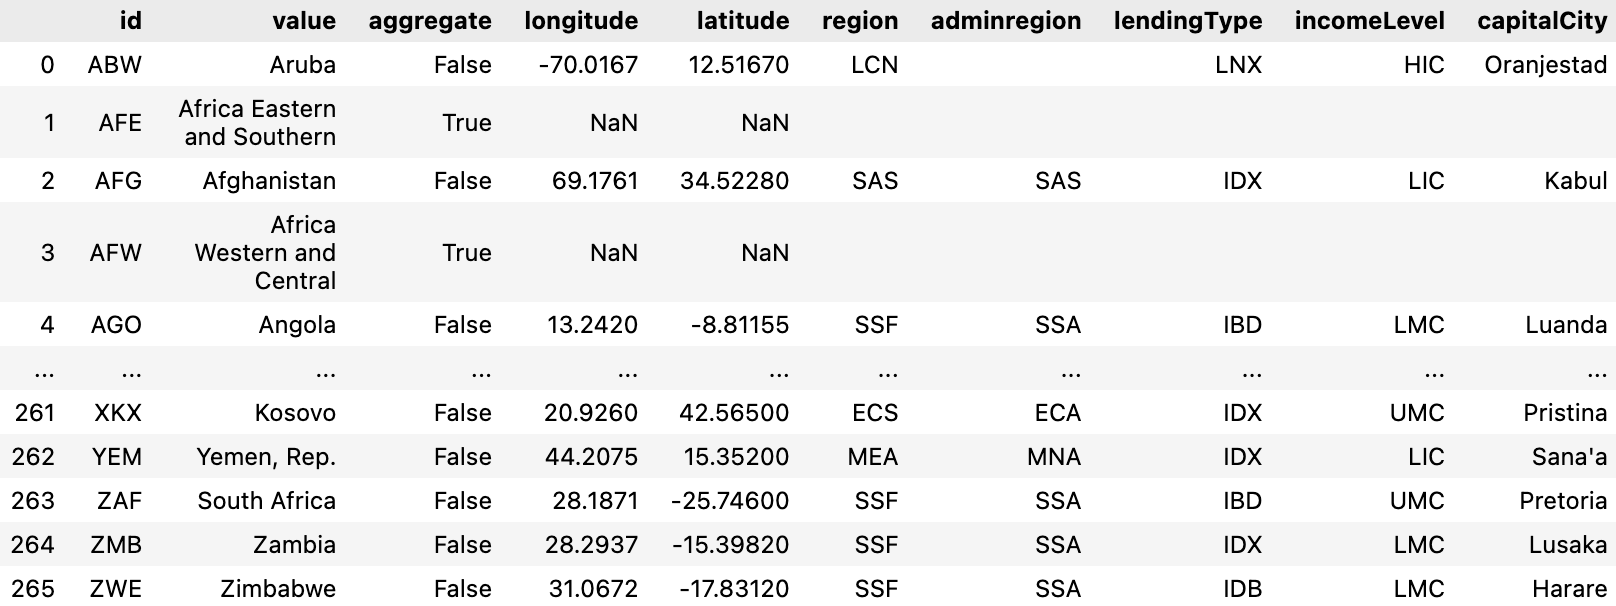
\includegraphics[width=0.9\textwidth]{economies.png}
  \caption{Economías World Bank}
  \label{fig:economies}
\end{figure}

Cada tópico tiene factores asociados:

\begin{figure}[htbp!]
  \centering
  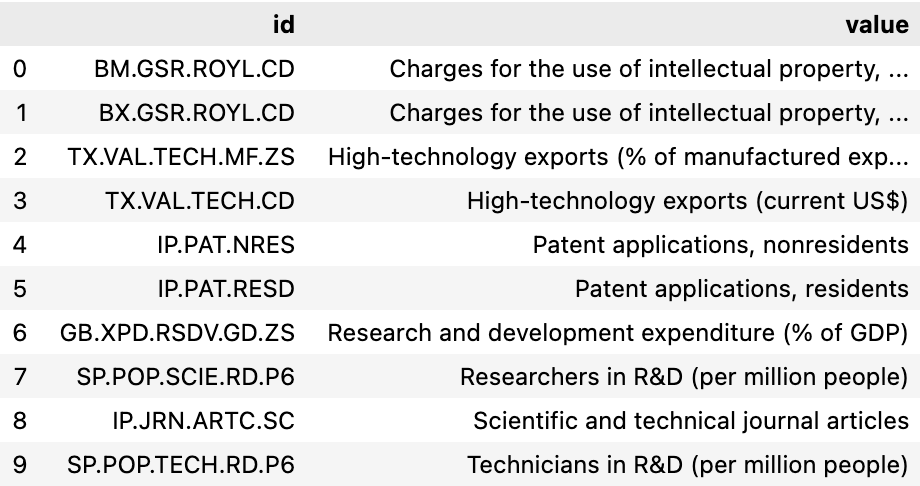
\includegraphics[width=0.7\textwidth]{st_factors.png}
  \caption{Factores Ciencia y Tecnología World Bank}
  \label{fig:stfactors}
\end{figure}

%%%%%%   Tópicos Posibles %%%%%% 

\subsection{Tópicos Posibles}

Contando valores faltantes:

\begin{figure}[htbp!]
  \centering
  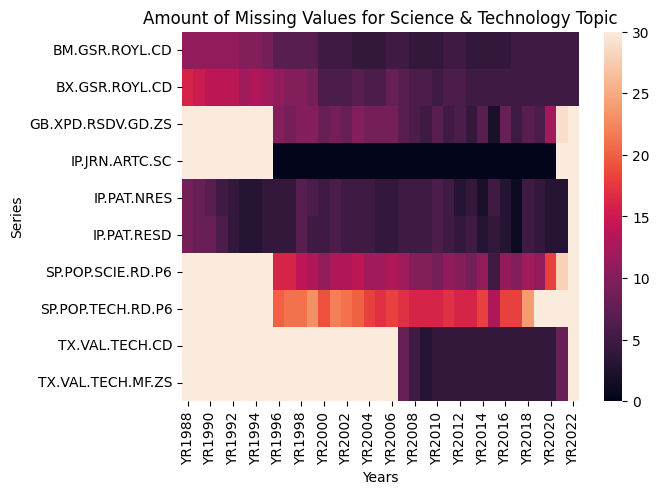
\includegraphics[width=0.7\textwidth]{Nan.png}
  \caption{Análisis de valores Nan}
  \label{fig:nan}
\end{figure}

\clearpage
\section{Stack Tecnológico} 

Hemos diseñado cuidadosamente nuestro stack tecnológico en base a la experiencia previa en estas herramientas y, lo que es más importante, en el valor que aportarán a nuestro proyecto.

Comencemos con el corazón de cualquier proyecto de data science: el lenguaje de programación. En este caso, hemos elegido Python. ¿Por qué Python? Primero y ante todo, es ampliamente utilizado en data science debido a su rica colección de bibliotecas. Pero más allá de su popularidad, es el lenguaje con el que estamos más familiarizados. Durante nuestra carrera, hemos trabajado extensamente con Python, lo que nos brinda la confianza necesaria para aprovechar al máximo sus capacidades y lograr un rendimiento óptimo en nuestro proyecto.

Para trabajar en este entorno, hemos optado por dos herramientas que consideramos esenciales: Visual Studio Code y Jupyter Notebook. Estas no son elecciones aleatorias, sino que se basan en nuestra experiencia previa. Visual Studio Code es un entorno de desarrollo altamente personalizable y eficiente, ideal para la escritura de código y la gestión de proyectos. Por otro lado, Jupyter Notebook es perfecto para la exploración de datos y la creación de informes interactivos. Al usar estas herramientas, podemos maximizar nuestra productividad y colaboración en el proyecto.

En cuanto a librerías y frameworks, hemos seleccionado las que se han convertido en pilares de data science. NumPy y pandas son esenciales para la manipulación y el análisis de datos, mientras que scikit-learn es nuestro aliado para el machine learning y el modelado. Además, Matplotlib y Seaborn son nuestras herramientas de confianza para la visualización de datos, permitiéndonos comunicar de manera efectiva los resultados de nuestro análisis.

Pero, ¿cómo compartiremos estos resultados? Aquí es donde Power BI entra en juego. Esta potente herramienta nos permitirá crear visualizaciones avanzadas y paneles interactivos, brindando un valor adicional a nuestros informes y ayudando a las partes interesadas a comprender mejor los resultados.

La gestión de proyectos es una parte crucial de cualquier emprendimiento. Para este propósito, hemos optado por Trello, una herramienta de seguimiento de tareas ágil y sencilla. Y, por supuesto, GitHub será nuestro centro de control de versiones y colaboración en código. No solo nos brinda un control de versiones sólido, sino que también nos permite mantener una documentación completa del proyecto, lo que es esencial para la reproducibilidad y la colaboración efectiva. Por último, Monday. Esta plataforma nos permite llevar de forma organizada nuestro diagrama de Gantt. 

En lo que respecta a la infraestructura y el alojamiento de recursos, hemos elegido Google Cloud Platform (GCP). GCP nos proporciona una infraestructura sólida y servicios en la nube que son esenciales para alojar nuestros datos y recursos, asegurando que estén disponibles cuando los necesitemos.

Finalmente, la comunicación y la colaboración son fundamentales para el éxito de cualquier proyecto. Por eso, utilizaremos Slack para la comunicación en equipo, Google Meet para nuestras reuniones y Presentaciones de Google para colaborar en tiempo real en documentos.

En resumen, hemos construido nuestro stack tecnológico cuidadosamente, aprovechando nuestra experiencia y seleccionando las herramientas que consideramos más adecuadas para nuestro proyecto de data science. Al hacerlo, estamos seguros de que maximizaremos nuestra eficiencia y efectividad, permitiéndonos abordar los desafíos que se presenten en el camino.

\begin{enumerate}
  \item Lenguaje de Programación
  \begin{itemize}
    \item Python
  \end{itemize}
  \item Entorno de Desarrollo
  \begin{itemize}
    \item Visual Studio Code 
    \item Jupyter Notebook
  \end{itemize}
  \item Librerías y Frameworks
  \begin{itemize}
    \item NumPy
    \item Pandas
    \item scikit-learn
    \item Matplotlib
    \item Seaborn:
  \end{itemize}
  \item Herramientas de Visualización
  \begin{itemize}
   \item Matplotlib
   \item Seaborn
   \item Power BI
  \end{itemize}
  \item Herramientas de Gestión de Proyectos
  \begin{itemize}
   \item Trello
   \item GitHub
   \item Monday
  \end{itemize}
  \item Infraestructura y Cloud
  \begin{itemize}
    \item Google Cloud Platform (GCP)
  \end{itemize}
  \item Comunicación y colaboración
  \begin{itemize}
    \item Slack
    \item Meet
    \item Presentaciones de Google
  \end{itemize}
\end{enumerate}


\clearpage
\section{Desarrollo del Proyecto} 
\subsection{Roles del Equipo}
\begin{table}[H]
  \centering	
  \caption{Roles del Equipo}
  \begin{tabular}{|p{5cm}|p{10cm}|}
    \hline
    \textbf{Role} & \textbf{Name} \\\hline
    Machine Learning & Gonzalo Ducca \\\hline
    Machine Learning & Carlos Madoery \\\hline
    Data Analytics & Valentino Caputa \\\hline
    Data Analytics & Juan P. Bertone \\\hline
    Data Engineer & Juan E. Flórez-Coronel \\\hline
  \end{tabular}
  \label{tab:teamroles}
\end{table}
\subsection{Diagrama de Gaant}
\begin{figure}[htbp!]
  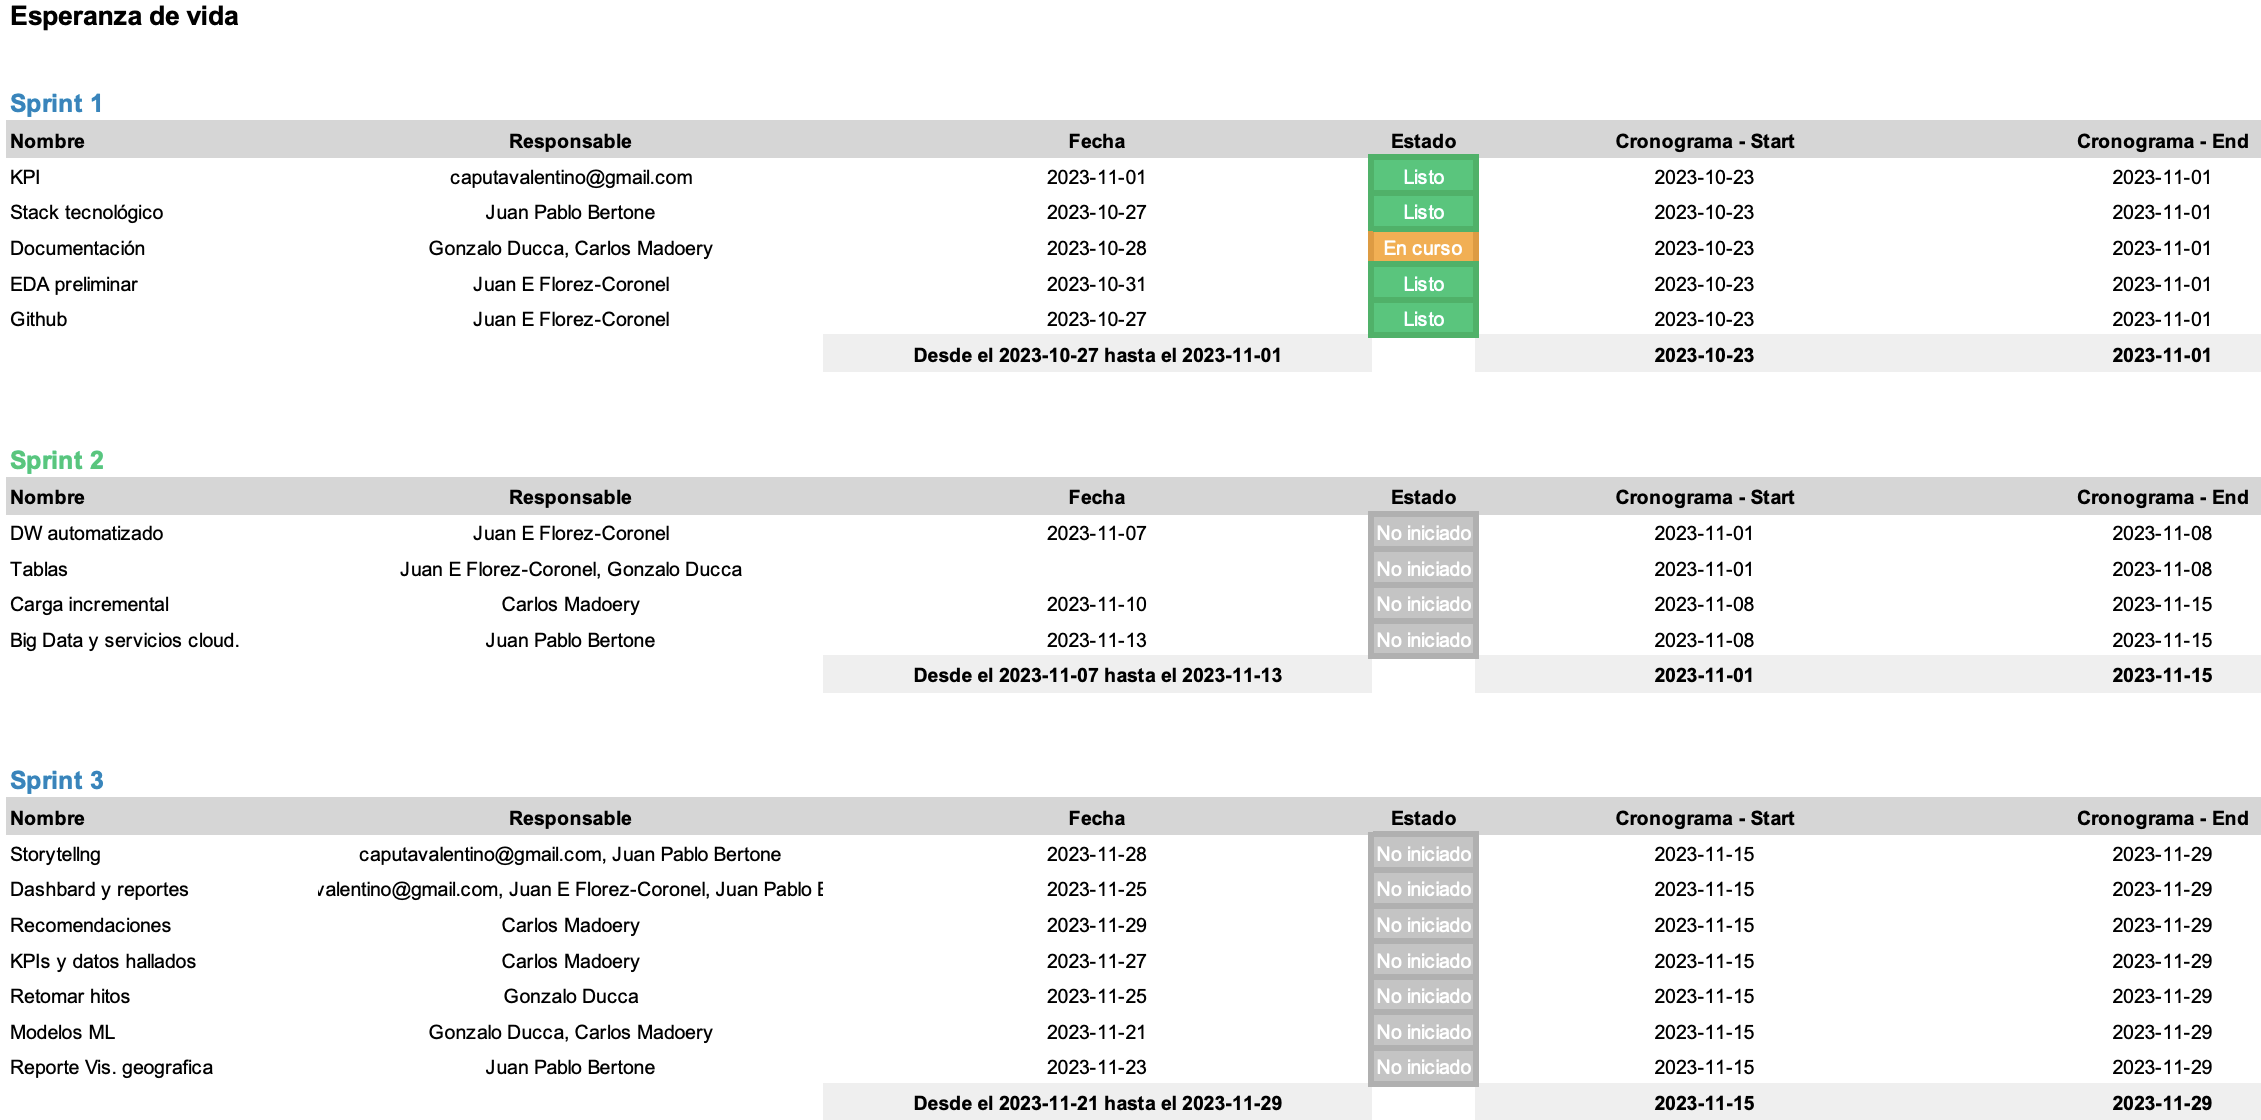
\includegraphics[width=\textwidth]{gaant.png}
  \caption{Diagrama de Gantt}
  \label{fig:gaant}
\end{figure}

\subsection{Demo 2}

Hasta el sprint anterior trabajamos sobre los objetivos y alcance del proyecto, el stack tecnológico implementado, la elaboración de un EDA preliminar, determinar los KPIs y la construcción de un diagrama de Gantt que nos permita organizar el plan de trabajo.
En esta nuevo demo se abordará: la realización de las bases de datos y el DER, el flujo de los datos, el servicio Cloud implementado junto a la carga incremental de los datos, un mockup de dashboard y una idea general sobre el modelo de Machine Learning que ofreceremos cómo producto al cliente.
El origen de las bases de datos es World Bank. Se eligieron 5 tópicos principales que consideramos afectan directamente a la esperanza de vida de un país: economía, educación, salud, desarrollo social y ciencia y tecnología. Vinculados a estos tópicos elaboramos los KPIs y se tomaron indicadores entre los que se encuentran: gasto público en educación, total (\% del PIB), esperanza de vida al nacer (años), prevalencia de la desnutrición (\% de la población), gasto en investigación y desarrollo (\% del PIB), homicidios intencionados (por cada 100.000 personas), entre otros.
Nos encontramos que muchos de los indicadores presentaban nulos en el primer intervalo de años o en la totalidad de los 30 años a estudiar, motivo por el cual decidimos descartar algunos.
A la hora de elaborar el diagrama entidad-relación, se construyeron 4 tablas: 1 de hechos y 3 de dimensiones. Inicialmente se confeccionó una tabla para ser usada con el modelo ML que contenía los indicadores en la columnas y pensarla cómo tabla de hecho, pero se decidió modificarla con las columnas  id, id\_pais, id\_indicador, año y valor. Continuando con el DER, se visualizan 3 tablas dimensionales: pais (id\_pais, nombre, longitud, latitud, región, capital), indicador (id\_indicador, id\_topico y descripción) y tópico (id\_topico, nombre).

\subsection{Google Cloud Platform}

\subsubsection{Justificación}

La decisión de implementar Google Cloud Platform (GCP) en nuestro entorno de trabajo responde a una estrategia destinada a optimizar el trabajo colaborativo. A continuación, se presentan algunas justificaciones clave para esta elección:

\begin{enumerate}
\item Escalabilidad y Flexibilidad Google Cloud Platform ofrece una arquitectura altamente escalable que nos permite ajustar nuestros recursos de manera dinámica según los objetivos y requisitos del trabajo.  
\item Amplio Conjunto de Servicios GCP proporciona una amplia gama de servicios en la nube que abarcan desde cómputo, almacenamiento y bases de datos hasta inteligencia artificial, aprendizaje automático y análisis de datos. 
\item Seguridad y Cumplimiento La seguridad es una prioridad fundamental, y GCP ofrece robustas medidas de seguridad para proteger nuestros datos y aplicaciones. 
\item Colaboración y Conectividad GCP facilita la colaboración entre equipos al proporcionar herramientas y servicios diseñados para un desarrollo ágil y una integración continua.
\item Innovación Continua GCP se caracteriza por su compromiso con la innovación constante. Al adoptar esta plataforma, nos aseguramos de tener acceso a las últimas tecnologías y actualizaciones, lo que nos permite mantenernos a la vanguardia en un entorno tecnológico en constante evolución.
\end{enumerate}

\subsubsection{Implementación}

En el contexto de nuestro trabajo práctico, hemos diseñado una estrategia integral que involucra tanto los servicios de Google Cloud Platform (GCP) como la integración de la API de World Bank. A continuación, se detalla la estructura de nuestra implementación:

\begin{enumerate}
  \item API de World Bank En primer lugar, optaremos por la integración de la API de World Bank, la cual nos proporcionará un acceso directo y actualizado a los datos. 
  \item Cloud Storage Como componente esencial, emplearemos Cloud Storage para almacenar de manera segura y eficiente los datos recopilados a través de la API de World Bank. Será nuestro Data Lake, donde la información se encontrará almacenada tal cual se recibe de la API. La API será invocada con una frecuencia de 4 semanas, con el objetivo de mantener la base actualizada. 
  \item Cloud Functions: La capa de automatización estará respaldada por Cloud Functions, permitiéndonos ejecutar código sin servidor de manera eficiente. Al aprovechar este servicio, garantizamos la automatización de procesos clave en respuesta a eventos específicos, asegurando una operación fluida y eficiente de nuestro sistema. Cada vez que los archivos se actualicen por la invocación a la API, se dispararán las funciones del cloud. Estas funciones tienen la tarea de realizar la limpieza de los datos y de trasnferirlos en el formato de tabla a BigQuery. 
  \item BigQuery Como motor SQL, BigQuery continuará desempeñando un papel fundamental en nuestro enfoque. La información almacenada en el motor mediante las funciones del cloud será el punto de partida para el análisis de los datos y la generación de modelos. 
  \item Looker Studio La fase final de nuestra implementación involucrará Looker Studio para la visualización y presentación de resultados. Looker Studio nos brindará la capacidad de crear paneles visuales intuitivos, facilitando la interpretación y comunicación efectiva de los hallazgos derivados de nuestros análisis.
\end{enumerate}

\subsection{Propuesta Machine Learning}

Se propone la creación de un modelo de Machine Learning (ML) destinado a predecir la esperanza de vida en un país determinado. Utilizando los indicadores definidos como el conjunto de variables predictoras.
El modelo buscará ofrecer una herramienta de predicción precisa y útil para diferentes audiencias, desde usuarios cotidianos hasta gobiernos interesados en comprender el impacto de cambios específicos en variables socioeconómicas.

La base técnica de nuestro modelo se fundamentará en el aprendizaje supervisado de regresión. Este tipo de modelo es idóneo para predecir valores continuos, como la esperanza de vida, a partir de variables predictoras. 

La entrada al modelo será una matriz de características que represente las variables predictoras definidas. Cada columna de esta matriz corresponderá a un indicador específico. 

El diseño del modelo contempla la posibilidad de incorporar variables categóricas. Las variables categóricas pueden proporcionar información adicional y enriquecer la capacidad predictiva del modelo. Por ejemplo, variables como la región geográfica, género o el sistema de gobierno podrían ser consideradas como variables categóricas que influyen en la esperanza de vida. Estas se codificarán adecuadamente para su inclusión en la matriz de características.

\textbf{Productos Diferenciados:}
El modelo de predicción se diseñará para producir dos resultados diferenciados, adaptados a distintas necesidades y audiencias:

\textbf{1- Producto para Usuarios Cotidianos:}
Este producto estará diseñado para satisfacer las necesidades de los usuarios cotidianos que desean conocer la esperanza de vida esperada en un país específico y en un año determinado. El input para este usuario será simple: el nombre del país y el año de interés. La interfaz será amigable y fácil de usar, proporcionando de manera clara y rápida la información buscada.

\textbf{2- Producto para Gobiernos:}
El segundo producto se orientará a gobiernos y entidades interesadas en entender el impacto de cambios específicos en las variables predictoras sobre la esperanza de vida. Permitirá definir ajustes porcentuales en una o más variables predictoras y visualizar la esperanza de vida resultante. Este enfoque proporcionará a los gobiernos una herramienta valiosa para la toma de decisiones informadas y la planificación estratégica.

\textbf{Beneficios y Aplicaciones:}
\begin{itemize}
  \item \textbf{Información Accesible:} Ofrecerá a los usuarios una visión rápida y accesible de la esperanza de vida, proporcionando información crucial para la planificación personal y la toma de decisiones informadas.
  \item \textbf{Planificación Estratégica:} Permitirá a gobiernos y entidades planificar estrategias basadas en la comprensión del impacto de cambios en variables socioeconómicas, facilitando la toma de decisiones y políticas más efectivas.
  \item \textbf{Adaptabilidad:} El modelo será diseñado para ser adaptable a diferentes contextos y regiones, brindando información valiosa a nivel global.
\end{itemize}



%%%%%%   Conclusiones  %%%%%%  
%\clearpage
%\section*{Conclusiones y Lecciones Aprendidas}
%\addcontentsline{toc}{section}{Conclusiones y Lecciones Aprendidas}%adds Conclusions and Lessons Learned section to the table of contents



%----References-----%
%\clearpage
%Please refer to the OverLeaf Primer to see your options for how to keep track of references.
%\section*{References}
%\addcontentsline{toc}{section}{References}%adds reference section to the table of contents
%Use the OverLeaf Primer to understand the different ways to format the references. 
%\bibliographystyle{IEEEtran} %Formats the bibliography to meet the IEEE standards
%\bibliography{ref.bib} %This command calls a file named "your_references.bib". You will upload this file, and can rename as necessary. 
  

%\clearpage
%\appendix
% \renewcommand{\thesection}{\Alph{section}.}
%\setcounter{section}{0}

%\addcontentsline{toc}{section}{Appendices}
%--Product System Design Decomposition----% 
%\section{Product System Design Decomposition}
%Provide a complete design decomposition. If the different branches relate to different parts of the product design (i.e safety, electrical subsystem, mechanical subsystem, etc...), please label those to show at a high level an overview of your decomposition. 

%Uncomment and use the below commands to include your decomposition. The "angle=90" rotates the decomposition to a landscape view. 

%-----------Figure------------%
% \begin{figure}[ht!]
% \centering
% \includegraphics[width=1.1\textwidth, angle=90]{Design_Decomposition}
% \caption{System Design Map}
% \label{System Design Map}
% \end{figure}
%-------End of Figure---------%


%--Design Drawings/Schematics----% 
%\clearpage
%\section{Design Drawings/Schematics}
%Please provide necessary drawings and schematics here. These should include both the mechanical and electrical figures if applicable. 


%----Appendix Proof of Material Purchase---% 
%\clearpage
%\section{Proof of Material Purchases}
%Please provide a copy of your receipt(s) for the purchase of the items on your bill of materials. 

%----Appendix: Other---% 
%\clearpage
%\section{Other}

\end{document}
